\documentclass[a4paper,11pt]{article}
\usepackage{indentfirst}
\usepackage[T1]{fontenc}
\usepackage[polish]{babel}
\usepackage[utf8]{inputenc}
\usepackage{lmodern}
\selectlanguage{polish}
\usepackage[top=2cm, bottom=2cm, left=1cm, right=1cm]{geometry}
\usepackage{lastpage}
\usepackage{fancyhdr}
\pagestyle{fancy}
\setlength\parindent{24pt}
\makeatletter
\newcommand{\linia}{\rule{\linewidth}{0.4mm}}
\renewcommand{\maketitle}{\begin{titlepage}
    \vspace*{2cm}
    \begin{center}\LARGE
    Politechnika Warszawska\\
    Wydział Elektryczny\\
    \end{center}
    \vspace{5cm}
    \noindent\linia
    \begin{center}
      \LARGE \textsc{\@title}
         \end{center}
     \linia
    \vspace{0.5cm}
    \begin{flushright}
    \begin{minipage}{5cm}
    \textit{Autor:}\\
    \normalsize \textsc{\@author} \par
    \end{minipage}
    \vspace{5cm}
     \end{flushright}
    \vspace*{\stretch{6}}
    \begin{center}
    \@date
    \end{center}
  \end{titlepage}
}
\makeatother
\author{Grzegorz Kopyt}
\title{Sprawozdanie \\
,,Arbitrage''}
\usepackage{graphicx}

\fancyhf{}
\rfoot{\thepage{}/\pageref{LastPage}}

\begin{document}
\maketitle

\tableofcontents
\vspace{1cm}
\noindent\linia
\section{Cel powstania dokumentu}
Dokument ma na celu podsumowanie pracy nad projektem ,,Arbitrage". Przedstawia problem, jaki miał zostać rozwiązany, opisuje zastosowany algorytm oraz wskazuje zmiany dokonane w stosunku do wcześniejszych specyfikacji. Dokument zawiera również wnioski z podjętych decyzji oraz refleksje nad zastosowanymi rozwiązaniami.

\noindent\linia
\section{Opis problemu}
Program został postawiony przed dwoma zadaniami:
\begin{itemize}
\item znajdowaniem najkorzystniejszej ścieżki wymiany waluty,
\item znajdowaniem dowolnego arbitrażu.
\end{itemize}

Jako źródło danych otrzymywał specjalnie spreparowany plik, który zawierał definicje walut oraz możliwych wymian (z informacją  o kursach i opłatach).
Na podstawie tego pliku oraz kwoty wejściowej program miał znajdować dowolny arbitraż. Natomiast do znalezienia najkorzystniejszej ścieżki wymiany waluty otrzymywał oprócz pliku i kwoty wejściowej, także walutę wejściową oraz docelową.

\noindent\linia
\section{Wysoko abstrakcyjny opis działania algorytmu}
\begin{enumerate}
\item Algorytm pobiera dane od użytkownika (w zależności od zadania są to dane opisane w sekcji 2).
\item Na podstawie tych danych algorytm tworzy graf walut, gdzie każda waluta zawiera możliwości jej wymiany na inną walutę.
\item Algorytm przechodzi kilkukrotnie po wszystkich walutach i możliwych wymianach (według algorytmu Bellmana-Forda) dokonując obliczeń wymiany określonej kwoty.
\item Jeśli znajdzie korzystniejszą ścieżkę dotarcia do węzła to aktualizuje jego dane.
\item W każdej walucie pozostawia największą kwotę oraz ścieżkę wymiany, którą można uzyskać z dotarcia do tej waluty od waluty początkowej.
\item W zależności od zadania:
\begin{enumerate}
\item Wymiana
\begin{enumerate}
\item Algorytm pobiera z waluty docelowej ścieżkę oraz kwotę końcową.
\end{enumerate}
\item Arbitrage
\begin{enumerate}
\item Algorytm pobiera z waluty początkowej, która jest także walutą końcową, ścieżkę wymiany oraz kwotę końcową.
\end{enumerate}
\end{enumerate}
\item Algorytm wyświetla użytkownikowi wyniki swojej pracy.
\end{enumerate}
\noindent\linia
\section{Efekty działania programu}
W wyniku pracy programu pojawiają się następujące sytuacje:
\begin{enumerate}
\item Poprawne wczytanie pliku.
\begin{center}
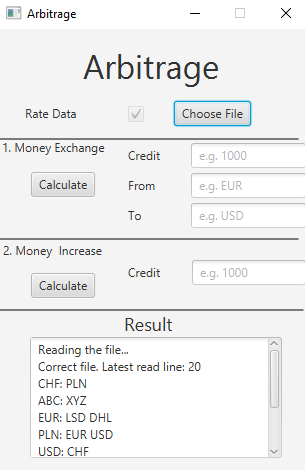
\includegraphics[width = 7cm]{DobryPlikWprowadzenie}
\end{center}
\item Niezgodność ze wzorem w pliku.
\begin{center}
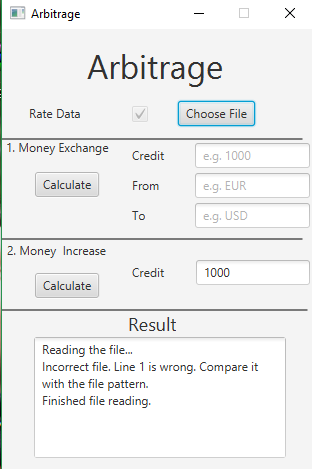
\includegraphics[width = 7cm]{badfilepattern}
\end{center}
\item Niepoprawny format pliku.
\begin{center}
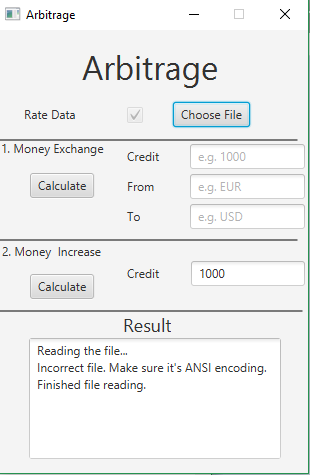
\includegraphics[width = 7cm]{badPlik}
\end{center}
\item Wybór pliku po naciśnięciu \textit{Choose File}.
\begin{center}
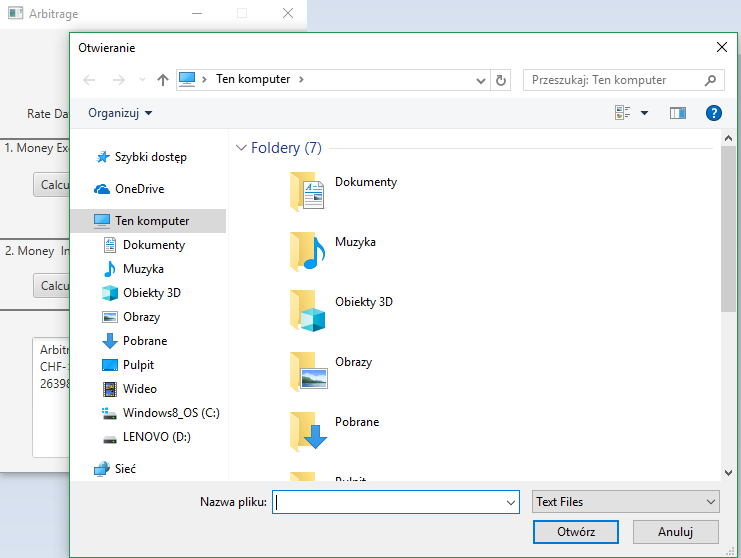
\includegraphics[width = 10cm]{filechooser}
\end{center}
\item Znalezienie arbitrażu.
\begin{center}
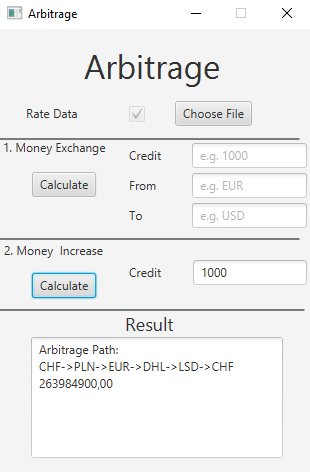
\includegraphics[width = 7cm]{DobryArbitrage}
\end{center}
\item Nie podano danych do wymiany lub arbitrażu.
\begin{center}
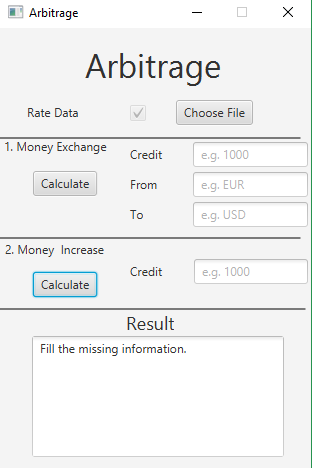
\includegraphics[width = 7cm]{NiePodanoDanych}
\end{center}
\item Znalezienie wymiany.
\begin{center}
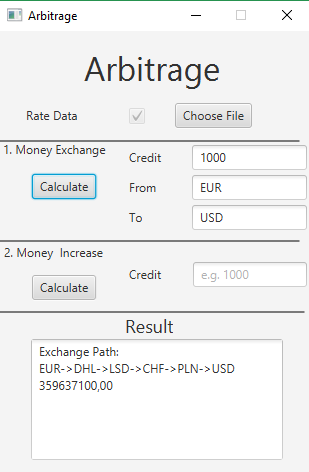
\includegraphics[width = 7cm]{DobraWymiana}
\end{center}
\item Podano za mało danych.
\begin{center}
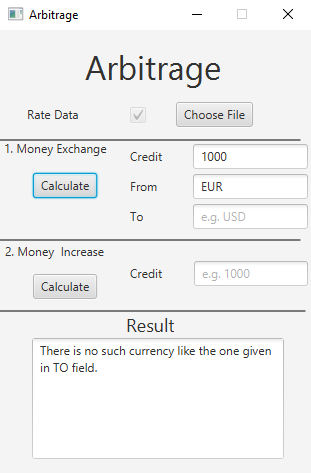
\includegraphics[width = 7cm]{ZaMaloDanych}
\end{center}
\item Nie podano pliku.
\begin{center}
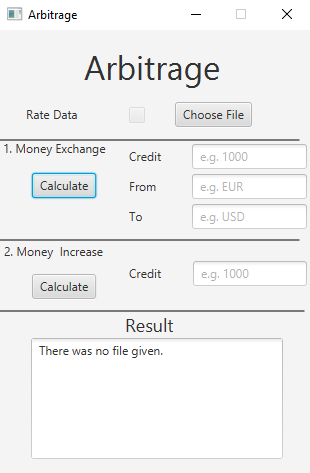
\includegraphics[width = 7cm]{nofilegiven}
\end{center}
\item Nie znaleziono arbitrażu.
\begin{center}
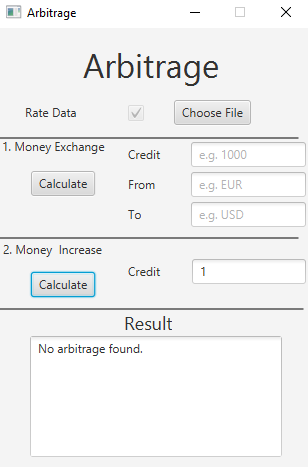
\includegraphics[width = 7cm]{noarbitrage}
\end{center}
\item Nie znaleziono wymiany.
\begin{center}
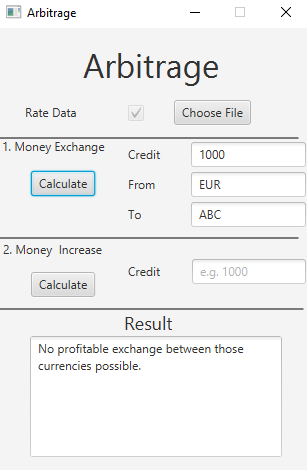
\includegraphics[width = 7cm]{noexchange}
\end{center}
\item Nie ma takiej waluty.
\begin{center}
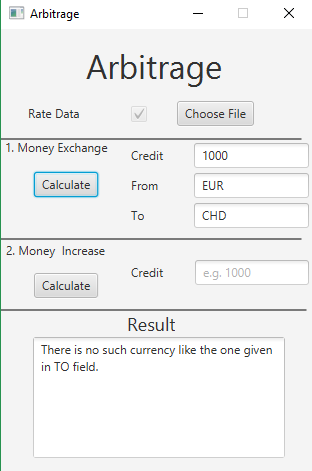
\includegraphics[width = 7cm]{nocurrency}
\end{center}
\end{enumerate}
\noindent\linia
\section{Zmiany względem specyfikacji}
\begin{enumerate}
\item Zmiana nazwy metody:
\begin{enumerate}
\item \textit{calculateProfitPath} na \textit{calculateArbitrage},
\item \textit{calculateExchangePath} na \textit{calculateExchange},
\item \textit{checkOfferLine} na \textit{checkRateLine}.
\end{enumerate}.
Zmiany te poprawiają czytelność kodu.

\item Zamiast jednej klasy \textit{GUI} powstał pakiet dwóch klas: \textit{Controller} i \textit{Main}.

Poprawia to czytelność kodu i wyodrębnia do klasy \textit{Controller} obsługę okna aplikacji.

\item Funkcjonalności klas \textit{FileChecker} i \textit{FileProcessor} zostały połączone w jedną klasę \textit{FileProcessor}.

Zmiana ta pozwala uniknąć podwójnego czytania pliku. W trakcie jednego czytania algorytm sprawdza jego poprawność oraz przetwarza zawarte w nim dane na graf.

\item Do obliczeń najkorzystniejszej ścieżki wymiany została dołączona także kwota początkowa.

\item Możliwa kwota wejściowa została ograniczona do prawie 10 miliardów (9 999 999 999,99).

Jest to arbitralnie przyjęta \textit{wystarczająco duża kwota} nie mniejsza od zarobków przeciętnego obywatela i~pozwalająca większości użytkowników swobodnie korzystać z funkcji programu.

\item Do \textit{FileProcessor} dodano pole \textit{repeatedCurrency}.

Ułatwia to przekazywanie użytkownikowi informacji o powtórzonej deklaracji tej samej waluty.

\item Do klasy \textit{Currency} dodano pole \textit{fullName} reprezentujące pełną nazwę waluty.

Pole to nie jest obecnie wykorzystywane, pozostaje w kodzie, ponieważ w przyszłości może okazać się przydatne do rozbudowy programu. Jest ono uzupełniane prawidłowymi wartościami z pliku wejściowego.

\item Została wydzielona klasa \textit{Graph}.

Powstała, aby uporządkować metody do operacji na mapie walut (\textit{currencies}), co poprawia czytelność kodu oraz łatwość korzystania z tych metod.
\item Do klasy \textit{Currency} dodano listę odwiedzonych walut.

Pozwala to na równoczesne znajdywanie ścieżki wymiany oraz kwoty docelowej.
\item Dodano klase \textit{LoopIterator}.

Klasa ta poprawia czytelność iteracji po węzłach (walutach) w sposób zgodny z algorytmem Bellmana-Forda (kiedy iterator dochodzi do końca tablicy wskazuje na jej zerowy element, co pozwala iterować po tablicy \textit{w~obiegu zamkniętym}).
\item Z uwagi na dodanie listy odwiedzonych węzłów do klasy \textit{Currency},  rola klasy \textit{Path} została zredukowana do nośnika informacji o ścieżce i kwocie końcowej.

\item W trakcie implementacji klasa \textit{FinancialAnalyst} okazała się niepotrzebnie wydzielona i została usunięta, ponieważ wszystkie jej domniemane funkcje spełnia klasa \textit{Broker}.
\item Zrezygnowano z obiektów \textit{CheckBox} w sekcji 1 oraz 2 okna aplikacji.

Obiekty te miały wskazywać, czy podano wartości do pól \textit{Credit}, \textit{To}, \textit{From}. Okazało się to niepotrzebne, ponieważ użytkownik jest w stanie zorientować się, czy pole zostało wypełnione, po samej zawartości pola.
\item Po poprawnym wczytaniu pliku program wyświetla informacje o walutach i ich możliwych wymianach.

Opcja ta została dodana, aby użytkownik mógł w łatwiejszy sposób sprawdzić jakie wymiany między walutami są dostępne.
\item Program dostosowany jest do czytania plików o kodowaniu ANSI.
\item Zostało przyjęte, że nazwy skrócone muszą być pisane wielkimi literami i składać się z 3 liter, dlatego, że jest to ogólnie przyjętym standardem.
\end{enumerate}
\noindent\linia
\section{Podsumowanie i wnioski}
Na implementacje algorytmu, wyszukującego arbitraż lub najkorzystniejsze wymiany walut miałem kilka pomysłów. Najbardziej oczywistym rozwiązaniem wydawało się zastosowanie algorytmu BFS albo DFS w celu odnalezienia wszystkich możliwych dróg w grafie między zadanymi walutami, a następnie wybranie tej najkorzystniejszej. Przed zastosowaniem jednego z tych algorytmów powstrzymywał mnie fakt, że znajdywanie wszystkich możliwych ścieżek w grafie wydawało mi się skrajnie nieefektywne, czasochłonne i niepotrzebne.

Zdecydowałem się na algorytm Bellmana-Forda, ponieważ bardzo spodobał mi się fakt, że po jednym jego wykonaniu wszystkie węzły zawierają informacje o koszcie dotarcia do nich. Dzięki temu użytkownik po ustaleniu waluty początkowej, może następnie dowolną ilość razy zmieniać walutę docelową, a algorytm i tak wykona operacje poszukiwania (ustawiania kosztów w grafie) tylko jeden raz. Przy każdym kolejnym żądaniu (dla tej samej waluty początkowej), będzie tylko pobierał z węzłów (walut) określone już ścieżki i kwoty. Decyzja ta oparta była również na moim osobistym przekonaniu, że przeciętny użytkownik jest w posiadaniu mniejszej ilości walut niż ilość tych walut, na które potencjalnie chciałby wymienić swoje pieniądze, czyli częściej będzie zmieniał walutę docelową niż wejściową.

W swojej implementacji tego algorytmu dokonałem zmiany polegającej na tym, że poszukiwany jest największy koszt dotarcia do węzła po ścieżce bez powtórzeń.

Algorytm prawidłowo wyznaczył ścieżki, we wszystkich przypadkach układu danych jakie testowałem. Poradził sobie zarówno w przypadku zapętlonych wymian jak i braku połączenia między walutami. Prawidłowo wyznaczył ścieżki w przypadku zróżnicowanych kursów i opłat jak i dla przypadku stałych opłat oraz kursów. Podołał w przypadku gęstych połączeń między węzłami jak i rzadkich. Arbitraż znalazł za każdym razem, gdy było to możliwe. Na podstawie przeprowadzonych przeze mnie testów działania algorytmu stwierdzam, że program działa prawidłowo.


Wnioski:
\begin{itemize}
\item algorytm Bellmana-Forda okazał się bardzo przydatny w realizacji tego zadania, pozwala zaoszczędzić wielu operacji;
\item ograniczenie nazw skróconych walut, nie pozwoli użytkownikowi na odejście od ogólnie przyjętych standardów oraz program przestanie być aktualny, jeśli standardy te ulegną zmianom;
\item algorytm jest uzależniony od osobliwego wzoru pliku, wartościową opcją rozwoju byłoby dodanie mu możliwość czytania plików w popularnym formacie jak np. JSON;
\item jednoczesne czytanie pliku oraz tworzenie grafu pozwala zaoszczędzić czas pracy programu, jednak utrudnia wymianę części programu odpowiedzialnej za tworzenie grafu bądź tej zajmującej się walidacją pliku.   
\end{itemize}

\noindent\linia

\end{document}



